\newpage
\section {Relatório de Setembro}

\subsection{Propostas para o mês:}
\begin{enumerate}
    \item Definição do oponente:
    \begin{itemize}
        \item Estudar e compreender o funcionamento das IAs.
        \item Definir as ações disponíveis para o oponente do jogador (por exemplo, se irá seguir as mesmas regras e limitações do player).
        \item Planejar como será seu baralho (se houver).
        \item Medir a dificuldade.
    \end{itemize}

    \item Programar a inteligência artificial:
    \begin{itemize}
        \item Programar sua racionalidade e decisões.
        \item Implementar sua interação com as cartas e com o jogador.
        \item Fazê-lo reagir às jogadas e mudanças de campo, tentando maximizar suas jogadas. 
    \end{itemize}
\end{enumerate}

\subsection{Atividades Realizadas:}

\subsubsection{Definição do Oponente}

Após algumas discussões, foi decidido o funcionamento da IA que controlará o oponente do jogador. Ela terá um campo extra de "\textit{background}", onde ficará as cartas que serão jogadas após liberar espaço em seu campo. Por exemplo, num campo 3x4 onde a primeira fileira (mais à baixo) é o campo do jogador, a do meio é as cartas "ativas" da IA (cartas nas quais ela pode agir) e a fileira de cima são as próximas jogadas da IA, que entrarão na fileira do meio assim que o espaço for liberado. Essa mecânica mais simples de oponente baseado em Inscryption é uma boa porta de entrada, mesmo que ainda não tenha uma racionalidade bem definida mas que pode ser aprimorada futuramente. 

\subsubsection{Andamento do Código}

O campo, como uma das partes mais importantes do jogo, está progredindo junto com alguns modelos iniciais para teste das entidades de carta e jogador. Sua estrutura inicial foi definida bem como alguimas funções principais e secundárias, como demonstrado a baixo.

\begin{figure}[htbp]
    \centering
    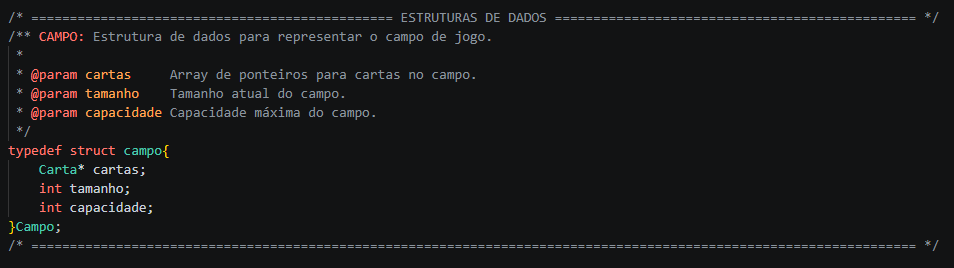
\includegraphics[width=1.0\textwidth]{estrutura-campo.png}
    \caption{Estrutura do campo.}
\end{figure}

\begin{figure}[htbp]
    \centering
    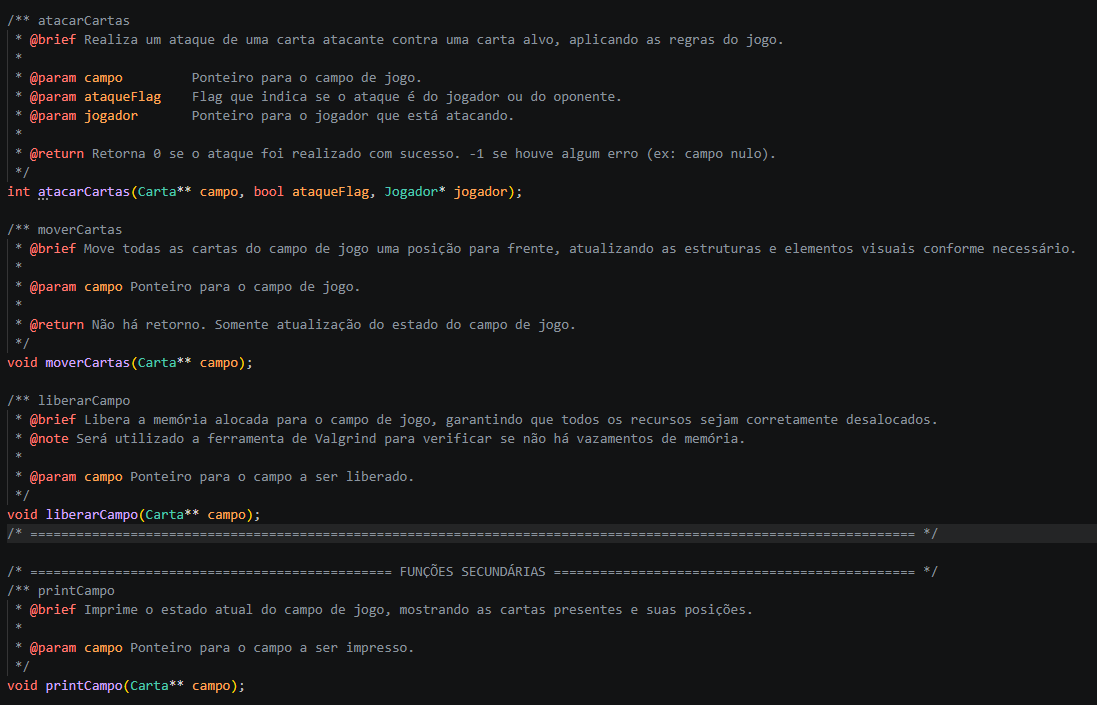
\includegraphics[width=1.0\textwidth]{print2.png}
    \caption{Funções principais.}
\end{figure}

\begin{figure}[htbp]
    \centering
    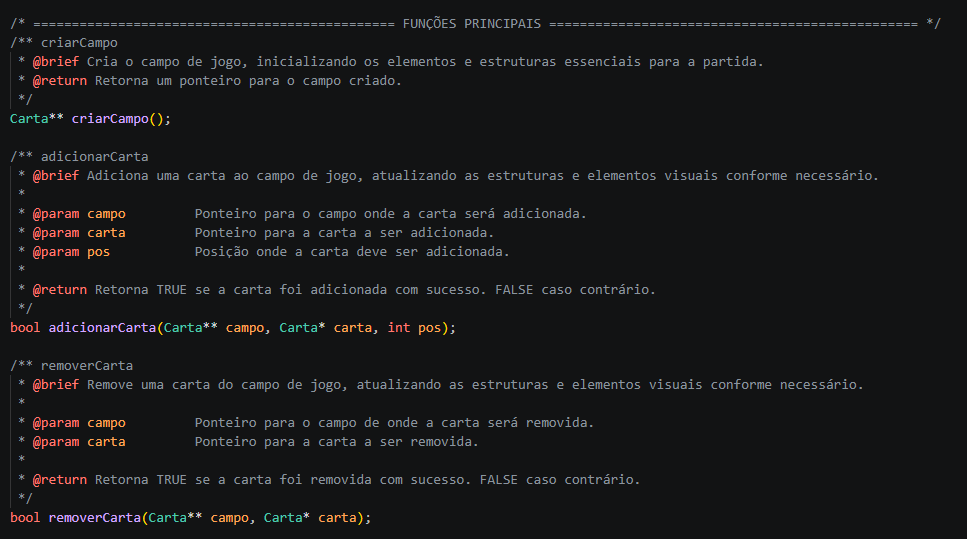
\includegraphics[width=1.0\textwidth]{print3.png}
    \caption{Funções principais e secundárias.}
\end{figure}

\begin{figure}[htbp]
    \centering
    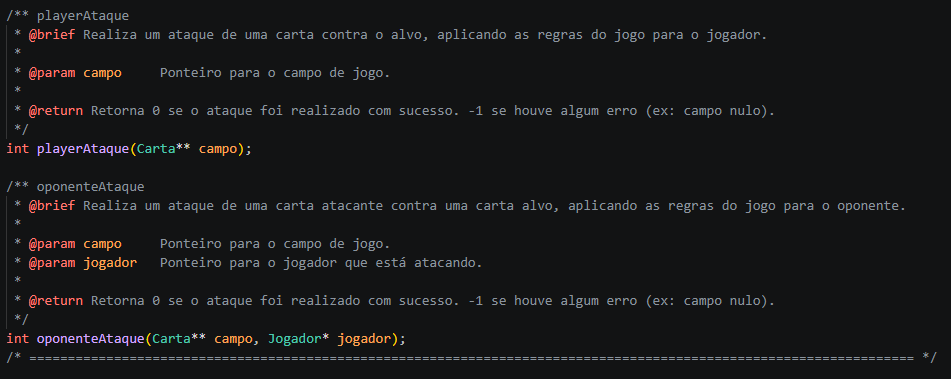
\includegraphics[width=1.0\textwidth]{print4.png}
    \caption{Mais funções secundárias.}
\end{figure}

\newpage

Como mencionado, algumas implementações para teste do campo foram feitas nos arquivos das cartas e jogador, como mostrado a baixo.

\begin{figure}[htbp]
    \centering
    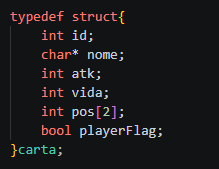
\includegraphics[width=1.0\textwidth]{estrutura-carta.png}
    \caption{Estrutura da carta.}
\end{figure}

\begin{figure}[htbp]
    \centering
    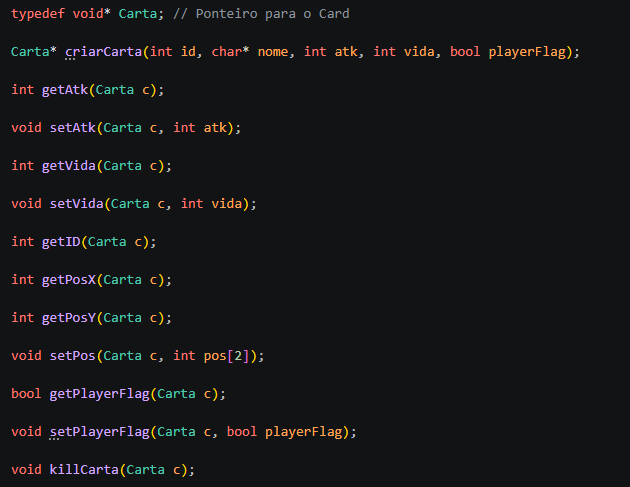
\includegraphics[width=1.0\textwidth]{print5.png}
    \caption{Funções iniciais da carta.}
\end{figure}

\begin{figure}[htbp]
    \centering
    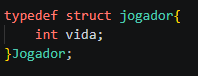
\includegraphics[width=1.0\textwidth]{estrutura-jogador.png}
    \caption{Estrutura do jogador.}
\end{figure}

\begin{figure}[htbp]
    \centering
    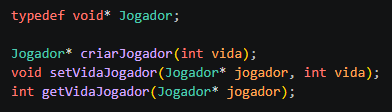
\includegraphics[width=1.0\textwidth]{print6.png}
    \caption{Funções iniciais do jogador.}
\end{figure}

\newpage

\subsubsection{Temática e Arte das cartas}

Mais artes das cartas estão sendo desenvolvidas, baseadas no modelo apresentado em reunião (figura a baixo). Tal modelo será um guia para as novas artes, demonstrando como deverá ser o estilo de arte bem como as informações da carta em sua imagem. Além disso, a temática do jogo para determinar seu estilo visual foi definido como "espaço", ou "astral".

\begin{figure}[htbp]
    \centering
    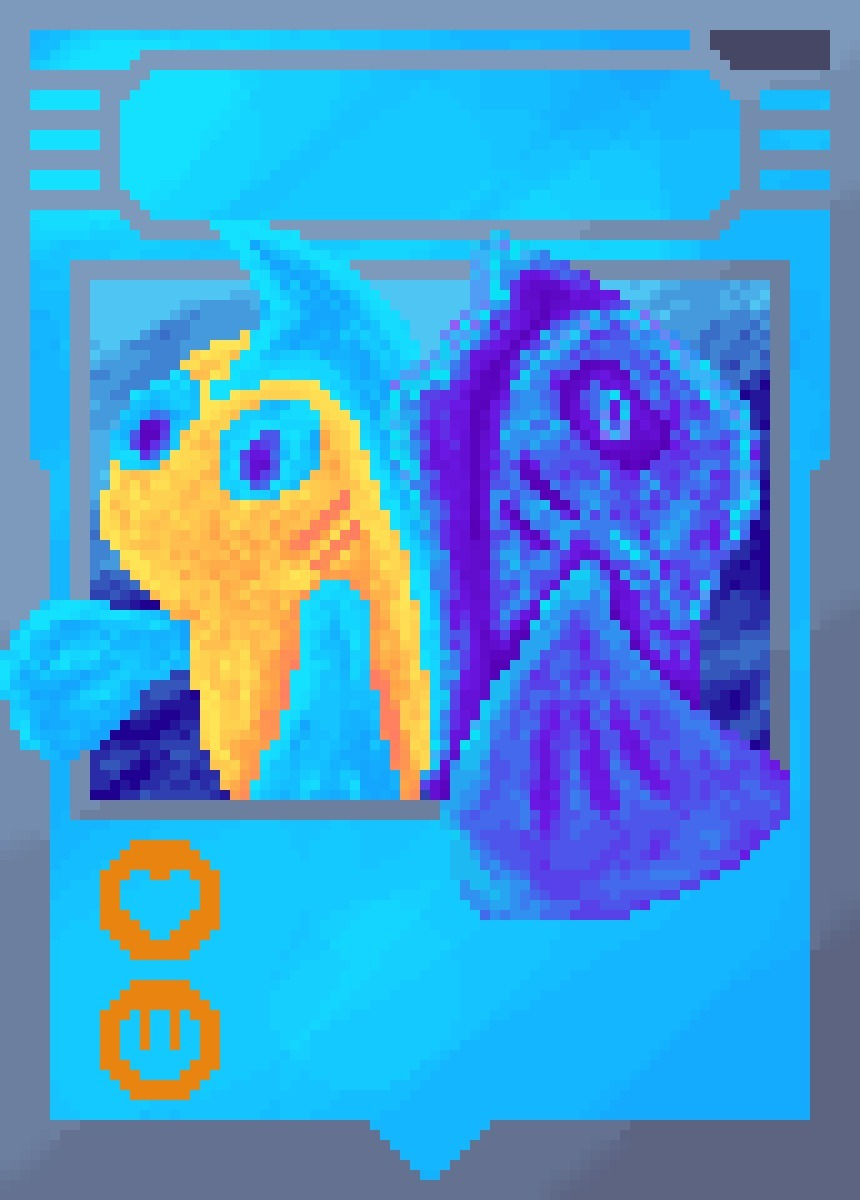
\includegraphics[width=0.7\textwidth]{carta-peixes.jpg}
    \caption{Exemplo do modelo e arte das cartas.}
\end{figure}

\newpage

Um \textit{placeholder} inicial para o menu principal também foi criado, com o nome do projeto estilizado e com fundo também pixelado.

\begin{figure}[htbp]
    \centering
    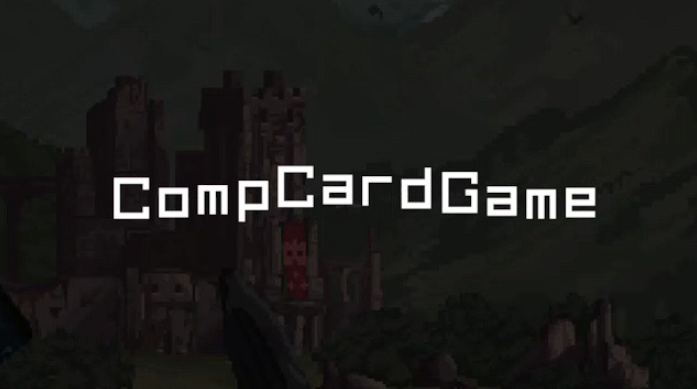
\includegraphics[width=0.7\textwidth]{tela-de-menu.png}
    \caption{Tela inicial de menu.}
\end{figure}

\subsubsection{Metas futuras}

Mesmo não tendo completado todas as metas, o jogo ainda está tomando forma e logo será jogável, sendo o próximo objetivo para o mês de Outubro. Também é esperado que novas cartas sejam feitas, para dar mais variedade no jogo e que elas sejam já funcionais nesse mês. 